%From: Pavel I Etingof <etingof@IAS.EDU>
%Date: Fri, 17 Jan 1997 18:49:14 -0500

\documentclass[11pt]{article}
 
\usepackage{amstex}
\usepackage[dvips]{epsfig}
 
\def\proclaim#1{{\bf #1} \it}
\def\endproclaim{\normalfont}
 
\def\tW{\tilde W}
\def\Aut{\text{Aut}}
\def\tr{{\text{tr}}}
\def\ell{{\text{ell}}}
\def\Ad{\text{Ad}}
\def\u{\bold u}
\def\m{\frak m}
\def\O{{\cal O}}
\def\tA{\tilde A}
\def\qdet{\text{qdet}}
\def\k{\kappa}
\def\RR{\Bbb R}
\def\be{\bold e}
\def\bR{\overline{R}}
\def\tR{\tilde{{\cal R}}}
\def\hY{\hat Y}
\def\tDY{\widetilde{DY}(\g)}
\def\R{\Bbb R}
\def\h1{\hat{\bold 1}}
\def\hV{\hat V}
\def\deg{\text{deg}}
\def\hz{\hat \z}
\def\hV{\hat V}
\def\Uz{U_h(\g_\z)}
\def\Uzi{U_h(\g_{\z,\infty})}
\def\Uhz{U_h(\g_{\hz_i})}
\def\Uhzi{U_h(\g_{\hz_i,\infty})}
\def\tUz{U_h(\tg_\z)}
\def\tUzi{U_h(\tg_{\z,\infty})}
\def\tUhz{U_h(\tg_{\hz_i})}
\def\tUhzi{U_h(\tg_{\hz_i,\infty})}
\def\hUz{U_h(\hg_\z)}
\def\hUzi{U_h(\hg_{\z,\infty})}
\def\Uoz{U_h(\g^0_\z)}
\def\Uozi{U_h(\g^0_{\z,\infty})}
\def\Uohz{U_h(\g^0_{\hz_i})}
\def\Uohzi{U_h(\g^0_{\hz_i,\infty})}
\def\tUoz{U_h(\tg^0_\z)}
\def\tUozi{U_h(\tg^0_{\z,\infty})}
\def\tUohz{U_h(\tg^0_{\hz_i})}
\def\tUohzi{U_h(\tg^0_{\hz_i,\infty})}
\def\hUoz{U_h(\hg^0_\z)}
\def\hUozi{U_h(\hg^0_{\z,\infty})}
\def\hg{\hat\g}
\def\tg{\tilde\g}
\def\Ind{\text{Ind}}
\def\pF{F^{\prime}}
\def\hR{\hat R}
\def\tF{\tilde F}
\def\tg{\tilde \g}
\def\tG{\tilde G}
\def\hF{\hat F}
\def\bg{\overline{\g}}
\def\bG{\overline{G}}
\def\Spec{\text{Spec}}
\def\tlo{\hat\otimes}
\def\hgr{\hat Gr}
\def\tio{\tilde\otimes}
\def\ho{\hat\otimes}
\def\ad{\text{ad}}
\def\Hom{\text{Hom}}
\def\hh{\hat\h}
\def\a{\frak a}
\def\t{\hat t}
\def\Ua{U_q(\tilde\g)}
\def\U2{{\Ua}_2}
\def\g{\frak g}
\def\n{\frak n}
\def\hh{\frak h}
\def\sltwo{\frak s\frak l _2 }
\def\Z{\Bbb Z}
\def\C{\Bbb C}
\def\d{\partial}
\def\i{\text{i}}
\def\ghat{\hat\frak g}
\def\gtwisted{\hat{\frak g}_{\gamma}}
\def\gtilde{\tilde{\frak g}_{\gamma}}
\def\Tr{\text{\rm Tr}}
\def\l{\lambda}
\def\I{I_{\l,\nu,-g}(V)}
\def\z{\bold z}
\def\Id{\text{Id}}
\def\<{\langle}
\def\>{\rangle}
\def\o{\otimes}
\def\e{\varepsilon}
\def\RE{\text{Re}}
\def\Ug{U_q({\frak g})}
\def\Id{\text{Id}}
\def\End{\text{End}}
\def\gg{\tilde\g}
\def\b{\frak b}
\def\S{{\cal S}}
\def\L{\Lambda}
 
 
 
 
\title {Lecture 3: Perturbative renormalization (continued)}
\author {Edward Witten}
 
\begin{document}
  
\begin{center}
{\LARGE\bfseries{Lecture 3: Perturbative renormalization (continued)} }\\
\vskip 1em%
{\Large Edward Witten}\footnote{\tt 
Notes by Pasha Etingof and David Kazhdan, TeXnical editing Misha Verbitsky} 
      \vskip 1.5em%
    {\large October 1996} \\ 
\end{center}
 

In this lecture we will discuss composite operators, their renormalization
and operator product expansion (OPE).

{\bf 3.1. Local functionals in a classical field theory.}

Consider an $n$-dimensional
 classical field theory with spacetime $V$ and a Lagrangian ${\cal L}$
of the form (2.3), with fields $\phi_1,...,\phi_N$. 
Let $X$ be the space of classical solutions for this theory.
We want to consider functions on $X$ called 
local functionals, which are defined as follows. 

Let $x\in V$ be a point in the spacetime. 

\proclaim{Definition} A local functional at $x$ is a function
of the fields and finitely many derivatives of the fields, evaluated at $x$. 
\endproclaim

{\bf Example} In the theory of a scalar bosonic field,
\[ \phi^l(x), \phi'(x)^2, \phi^2(x)\phi'(x)^2\] are local functionals,
but $\phi(x)+\phi(2x)$ is not. 

{}From the previous lecture it is clear how to define dimension of
a local functional. We want to consider only homogeneous 
functionals of finite dimension and their finite linear combinations. 
Therefore, if a field has positive dimension (which is always the case
if $n>2$), we only consider polynomial functionals of this field.
However, in 2-dimensional theories, where bosonic fields are 
dimensionless, it is reasonable and useful to consider
more general functions of them (for example, the Lagrangians of Toda theories
contain expressions of the form $e^\phi$).

If $n>2$, the space of all functionals of a given dimension 
is finite-dimensional, but if $n=2$, it is infinite-dimensional. 

Since elements of $X$ satisfy the classical field equations, 
the same local functional can be written in different ways. 
For example, in $\phi^4$-theory the classical field equation is
$$
\Delta\phi=m^2\phi+\frac{g}{3!}\phi^3,\leqno{(3.1)}
$$
so the left and the right hand sides of (3.1) evaluated at $x\in V$
represent the same local functionals of $\phi$. Thus, local functionals 
are all possible differential expressions in $\phi$ modulo 
the classical field equations. 

{\bf Remark 1.} One should be careful to 
distinguish between two different notions of field dimension
which arise in field theory. The first is ``the engineering dimension''
and says in what units the field is measured
(if the units are $cm^{-d}$ then the engineering dimension is $d$). 
The second is 
``the scaling dimension'', which is the dimension we have been talking about. 
These two dimensions are not always the same. 
For example, in the theory of one field $\phi$ defined by (3.1)
the engineering dimension of the field $m^2\phi$ is 3 (it is measured
in $cm^{-3}$), while the scaling dimension is the same as that of $\phi$, 
i.e. $1$. 

It is the basic principle of physics that all meaningful expressions 
and equations are homogeneous with respect to the engineering dimension. 
In particular, it is true for the field equations 
in field theory (e.g. (3.1)), 
which implies that engineering dimension defines a grading
on the space of local functionals. On the other hand, 
whenever a field theory is not scale invariant, 
its field equations are not homogeneous with respect to the scaling 
dimension,  so scaling dimension defines a filtration, rather than 
a grading, on the space of local functionals. This means, the space 
of all local functionals is a union of subspaces of functionals of dimension
$\le d$, and a functional is said to be of dimension $d$ if it is of 
dimension $\le d$ but not $\le d-1$. On the other hand, 
if the theory happens to be scale invariant, scaling dimension 
does define a filtration on the space of local functionals. 

In this lecture, we will not use engineering dimension, and the word 
``dimension'' will always mean scaling dimension. 

{\bf Remark 2.}  From a local functional $\O$ 
one can obtain more general functionals on $X$ of
the form $\int \O(\phi,x)d\mu(x)$, where $d\mu(x)$ is a (generalized) 
density on $V$. Using this operation, one can obtain from any local
functional all derivatives of thus functional (it is enough to 
take for $d\mu(x)$ all possible densities supported at $x$).
Therefore, without loss of information we could consider local functionals
modulo the image of derivatives. However, for the purposes of this lecture 
this is not necessary.   

{\bf 3.2. Quantization of local functionals in a free theory}

We have seen (see Bernstein's Lectures and Witten's problem sets) 
that the space $X$ 
of classical solutions of a meaningful classical field theory
always carries a natural closed 2-form $\Omega$. If this form is 
nondegenerate, $X$ is a symplectic manifold. In this case, suitable
functions on $X$ form a Poisson algebra. 

In the quantum theory, the space $X$ should be quantized, and
the Poisson algebra of functions on $X$ should become the algebra of
operators (observables) in some Hilbert space of states. 
In particular, we should be able to assign 
an operator to every local functional. 

If $V$ is a Minkowski space, and the field theory satisfies 
the Wightman axioms (for example, the free theory), 
the Hilbert space of states ${\cal H}$ is constructed as described
in Kazhdan's lectures. In this case, Wightman fields $\phi(x)$ are
distributions on $V$ with values in the space of operators 
on the subspace ${\cal D}\subset {\cal H}$
of muptiparticle states. 
This means, for any Schwarz function $f$ on $V$ 
there is an honest operator $\varphi(f)$ on ${\cal D}$. 

However, we would like to have more general operators of the form 
$\phi^N(x)$, $(\nabla\phi)^2(x)$, etc. which correspond 
to local functionals in the classical theory. That is, for any 
Schwarz function $f$ we want to have operators $\varphi^N(f)$, 
$(\nabla\varphi)^2(f)$, etc. 

Unfortunately, such operators are not automatically defined. 
For example, even $\varphi^2(f)$ does not, in general, 
make sense. Indeed, let $\delta_\e=e^{-|x|^2/\e}(2\pi/\e)^{n/2}$
be the smooth approximation to the $\delta$-function, and
let $\varphi\o\varphi$ be the operator-valued distribution on 
$V\times V$ given by $\varphi\o\varphi(f_1\o f_2)=
\varphi(f_1)\varphi(f_2)$. 
The natural definition of $\varphi^2(f)$ would be that $\varphi^2(f)$
is the limit, as $\e\to 0$, of 
the operator $\varphi_\e^2(f):=\varphi\o\varphi(f(x)\delta_\e(x-y))$ 
(in the sense of convergence of matrix elements). 
However, it is easy to see that this limit does not usually exist, as 
Wightman functions usually have singularities on the diagonals. 

One way to deal with this problem is to say that an ``operator''
$A$ is just a collection of its matrix elements, i.e. a collection
of correlation functions $\<\phi(y_1)...\phi(y_l)|A|\phi(z_1)...\phi(z_r)\>$. 
If we accept this point of view, we might as well forget about the Hilbert
space of states, i.e. perform a Wick rotation from Minkowski space to Euclidean
space, and consider Schwinger functions instead of Wightman functions. 

So from now on we will consider only the Euclidean situation, in which 
we will mean by an operator $A$ a collection of
functions \[ \<\phi(y_1)...\phi(y_l)|A|\phi(z_1)...\phi(z_r)\>\]
with certain properties. Roughly, an operator is just a symbol which can be
inserted in a correlation function. 

{\bf Remark.} 
Of course we should remember at all times that $A$ is not really an
operator and does not act in any Hilbert 
space. However, the information we get 
from studying $A$ in the Euclidean situation can be used (after Wick
rotation) for studying the Minkowski situation. 

Consider now the problem of quantization of local functionals. 
By the definition, in order to quantize the local functional $\O(x)$, we should
say what the functions 
$\<\phi(y_1)...\phi(y_l)|\O(x)|\phi(z_1)...\phi(z_r)\>$
are. As our theory is Euclidean, the order of factors in the correlation
function does not matter
(any two distinct points are space-like separated). 
So, in order to define $\O(x)$, it is enough 
to define the correlation functions $\<\phi(y_1)...\phi(y_r)\O(x)\>$
for all $r$. 

Consider the theory of a scalar bosonic field in $n>2$ dimensions, with the 
Lagrangian
$$
{\cal L}(\phi)=\int 
(\frac{1}{2}(\nabla\phi)^2+\frac{m^2}{2}\phi^2+Q(\phi))d^nx,\leqno{(3.2)}
$$
We will give all definitions and constructions for this example. 
In other field theories, everything is done in a similar manner. 

We first consider the case when the theory is free ($Q=0$).
In a free theory, quantization is done with the help of normal ordering, as
follows. Consider a local functional $\O$ of degree $J$ in $\phi$. 
According to Feynman rules, in order to compute the correlation 
function $\<\phi(y_1)...\phi(y_r)\O(x)\>$, we should consider 
all graphs with $r$ external vertices and only one internal vertex $v$,
which has $J$ edges. We should put a certain function at the
vertex $v$, and compute the term (amplitude) corresponding to this graph
as usual in Feynman calculus. If $J>1$, we will run into trouble: 
we will get some graphs with loops going from $v$ to itself, 
and the integration over the loops is divergent. 
The easiest remedy is to ignore all such graphs. Then we obtain 
certain correlation functions, which define some operator. This operator
is denoted by $:\O(x):$ and called the normal ordering of $\O(x)$. 
Apriori, $\O(x)$ does not make sense as an operator, while
$:\O(x):$ does. We call operators of the form $:\O(x):$
composite operators. When no confusion is possible, 
we will drop the dots and write $\O(x)$.  

Thus, we have assigned canonically to each differential polynomial $\O$ 
in $\phi$ an operator $:\O:$ in the free theory. 
However, recall that two different polynomials $\O_1,\O_2$ might 
define the same local functional. So does the map $\O\to :\O:$ actually define
canonically a quantization of the local functional represented by $\O$?
The answer turns out to be positive: whenever polynomials
$\O_1$, $\O_2$ define the same local functional, 
the operators $:\O_1:,:\O_2:$ coincide. 
To check this is an easy exercise.  For example, the polynomials 
$\O_1=\phi\Delta\phi$, $\O_2=m^2\phi^2$ define the same local functional, 
and the operators $:\phi\Delta\phi:$, $:m^2\phi^2:$ coincide. 

{\bf 3.3. Multiplication of composite operators.} 

It is easy to multiply composite operators supported at different points.
That means, given two composite operators $\O$, $\O'$, 
and points $x,x'\in V$, $x\ne x'$, it is easy to define
an operator $\O(x)\O'(x')$, using the Feynman diagram expansion. 
In this case we will have two special vertices $v,v'$, 
and we should sum over all ways of connecting them which involve no loops
from a vertex to itself.
However, multiplication of two composite operators $\O,\O'$
at the same point $x$ cannot be 
defined in the same way: on each edge connecting $v$ with $v'$, 
we will have to evaluate the Green's function at $(x,x)$, where it is 
singular. 

To avoid this problem, one can try to smear the operators, i.e. consider
the operator $\O(f)=\int f(x)\O(x)d^nx$, where $f$ is a compactly supported
smooth function on $V$. Such smeared operators can sometimes be
multiplied: for example, we can define the product $\phi(f_1)...\phi(f_s)$.
(see Kazhdan lectures).

However, most composite operators cannot be
multiplied, even after smearing. Indeed, 
it can be deduced from reflection positivity
that for any complex operator $\O$ 
$\<\O(x)\O^*(x')\>\sim |x-x'|^{-2[\O]}$, $x\to x'$ where
$[\O]$ is the dimension of $[\O]$, and $\O^*$ is the conjugate of $\O$. 
On the other hand, for a real operator $\O$,
in order for the product 
$\O(f)\O(f')$ 
to be defined, it is necessary and sufficient that 
the functions
$\<\phi(y_1)...\phi(y_r)\O(x)\O(x')\>$ be distributions. 
The function $|x|^{-l}$ defines a distribution 
(without regularization) if and only if 
it is locally $L^1$, i.e. iff $l<n$. Thus, the product 
$\O(f)\O(f')$ is automatically
defined iff $[\O]<n/2$. 

{\bf Remark.}
If the Minkowski situation, the product $\O(f)\O(f')$
exists (in the sense of correlation functions) 
if and only if the ``operator'' $\O(x)$ is an operator-valued
distribution, so that  
$\O(f)$ is actually an honest operator (i.e. matrix elements
of $\O(f)$ are matrix elements of some operator on ${\cal D}$).
Indeed, the ``if'' part is clear. The ``only if'' part: 
for any $f_1,...,f_N$ we can regard the product 
$X=\O(f)\varphi(f_1)...\varphi(f_N)$ as a linear functional on ${\cal D}$.
The fact that $\O(f)^2$ is defined implies that this functional
has finite $L^2$-norm, as $||X||^2=
\<\varphi(f_N)...\varphi(f_1)
\O(f)^2\varphi(f_1)...\varphi(f_N)\>$. Therefore, $X$ corresponds to 
a vector in ${\cal H}$, Q.E.D.

{\bf 3.4. Operator product expansion (OPE) in the free theory}

Composite operators in a reasonable field theory have an important
algebraic property, which is called the operator product expansion (OPE).
This is a property of algebraic nature, saying roughly that composite
operators form an algebra of a certain kind. It does not follow 
obviously from Wightman axioms, but on the other hand
is often satisfied when Wightman axioms fail. This property is
actually useful in practice. 

We will now define and compute 
the OPE for the free theory of a scalar bosonic field. 
The idea is to formalize the behavior of the product $\O(x)\O'(x')$
as $x\to x'$. In the classical theory, this is accomplished by
the usual Taylor
series.
Indeed, we have
$$
\O(x)\O'(x')=\O(x')\O'(x')+(x-x')_\mu\d_\mu\O(x')\O'(x')+...\leqno{(3.3)}
$$
Thus, for any two local functionals
$\O,\O'$ the product $\O(x)\O'(x')$ decomposes in a series in products
of powers of $(x-x')_\mu$ whose coefficients are other local functionals.

In the quantum theory, the product $:\O(x)::\O'(x'):$, as we have seen, is 
singular at $x=x'$. Thus, we have to compute the asymptotic expansion
of this product near $x=x'$.

We will assume that $\O,\O'$ are 
represented by some monomials in $\phi$ and its derivatives. 
According to Feynman rules, we should assign to both $\O,\O'$ a vertex,
say $v$ and $v'$. The numbers of edges at $v,v'$ are $J,J'$, where
 $J,J'$ are the degrees of $\O,\O'$ as monomials
of $\phi$. At both $v,v'$, we have to place symmetric distributions 
in $J,J'$ variables corresponding to $\O,\O'$. Now we have to sum amplitudes
over all ways of connecting some edges going from $v$ with some edges
going from $v'$. The amplitude of each particular graph is computed as 
follows: at each edge going from $v$ to $v'$ we put the function
$D(y-z)$, the two-point Schwinger
function of the free theory (the Green's function for the Helmholtz 
equation). 
On each remaining external edge we put
$\phi(y)$. Then we compute formally the product
of things on vertices and edges, and put it under the normal ordering
sign. Since for each number $K$ of connecting edges, we have only one possible
graph, we should just compute the amplitude of this graph, and 
then multiply it by the number of ways to get this graph, i.e. by
$J!J'!/K!(J-K)!(J'-K)!$. 

This will give us a formula of the form
$$
:\O(x)::\O'(x'):=\sum_{k=1}^L:\tilde\O_k(x)\tilde\O_k'(x'):E_k(x-x'),\leqno{(3.4)}
$$
where $:\tilde\O_k:,:\tilde\O_k':$ are some local functionals, and
$E_k(y)$ are polynomial differential operators in $D(y)$.
Here $:\O(x)\O'(x'):$ is the amplitude of the graph in which 
the vertices $v$ and $v'$ are not connected. 

Now we can use the Taylor formula (3.3) inside of the normal 
ordering, to get the following (already infinite) expansion:
$$
:\O(x)::\O(x'):=\sum_s :\O_s(x'):D_s(x-x'),\leqno{(3.5)}
$$
where $\O_s$ is local functional, and $D_s(y)$ is a product
of the function $E_k(y)$ for some $k$ and a polynomial in $y$.  

{\bf Definition.} Expansion (3.5) is called the operator
product expansion (OPE). 

Now recall that the Green's function $D(x)$ has the following behavior
at $x=0$: $D(x)\sim |x|^{2-n}$. Therefore, all functions
$d_k(x)$ have the property $|d_k(x)|\le C_k|x|^{r_k}$ for small $x$, where
the numbers $r_k$ are almost all positive. This proves an important
property of the OPE: only finitely many terms are singular. 
However, these singular terms carry the most interesting information
in many situations. 

{\bf Remark.} We see that the 
operator product expansion (3.5) is in fact the quantum analogue of the Taylor
expansion (3.3). Indeed, it is an expansion of the form similar to (3.3),
but also involving finitely many singular terms at $x=x'$. 

Let us now consider examples of OPE (we will always write the finite
formula (3.4)). 
Let us first compute $\phi(x)\phi(x')$. 
Using the above rules, we get two graphs:

\begin{center} 
 
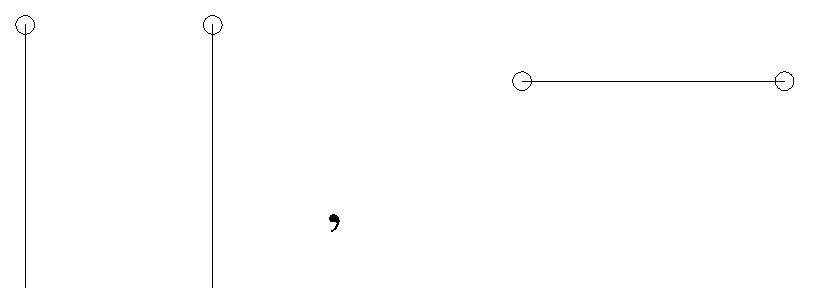
\epsfig{file=lec3-page5-1.eps,width=.4\linewidth} 
 
\end{center}


which yields the formula
$$
\phi(x)\phi(x')=:\phi(x)\phi(x'):+D(x-x').\leqno{(3.6)}
$$
Now we compute $:\phi^2(x)\phi^2(x'):$.
This product gives us three graphs:


\begin{center} 
 
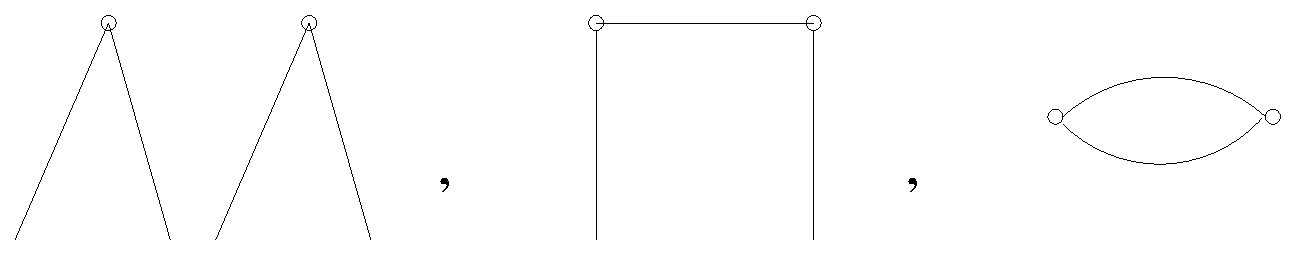
\epsfig{file=lec3-page5-2.eps,width=.5\linewidth} 
 
\end{center}


so we get the formula
$$
:\phi^2(x)::\phi^2(x'):=:\phi^2(x)\phi^2(x'):+4:\phi(x)\phi(x'):
D(x-x')+2D^2(x-x').\leqno{(3.7)}
$$
In general, it is easy to prove that
$$
\begin{aligned}:\phi^J(x)::\phi^{J'}(x'):=&
\sum_{K=0}^{\min(J,J')}\frac{J!J'!}{K!(J-K)!(J'-K)!}\times \\&\times
D(x-x')^K:\phi^{J-K}(x)\phi^{J'-K'}(x'):\end{aligned}\leqno{(3.8)}
$$
The last formula can be written more nicely using generating functions:
$$
\begin{aligned}
:e^{\alpha \phi(x)}::e^{\beta \phi(x')}:=
e^{\alpha\beta D(x-x')}:e^{\alpha\phi(x)}e^{\beta\phi(x')}:,
\end{aligned}\leqno{(3.9)}
$$
where $\alpha,\beta$ are constants.

If we take $\alpha,\beta$ to be any differential operators 
on $V$ with constant coefficients,
this formula remains valid. 
($\alpha$ acts on $x$, $\beta$ on $x'$). 
In this form, formula (3.7) represents the most general
OPE for the free theory of a scalar bosonic field. 

{\bf Remark.} Dimensions of fields in quantum theory may differ
from the dimensions of their classical analogues. For example, 
in a (2-dimensional) classical field theory, if a field $\phi$ is
0-dimensional, so is $f(\phi)$, where $f:\R\to\R$ is any function. 
However, in quantum theory a renormalized composite operator $f(\phi)$ 
may acquire a nontrivial (anomalous) dimension. For example, 
in the free 2-dimensional theory of a massless scalar bosonic field,
$D(y)=-\ln|y|$, so we have from (3.9):
$$
\<:e^{i\alpha\phi(x)}::e^{-i\alpha\phi(y)}:\>=|x-y|^{-\alpha^2}.
$$
But we know that $\O(x)\O^*(y)\>\sim |x-y|^{-2[\O]}$. 
Thus, the scaling dimension of $e^{i\alpha \phi}$ is $d(\alpha)=\alpha^2/2$. 
Observe that the function $d$ is not linear in $\alpha$, 
so for quantum dimensions, to the contrary with the classical dimensions,
 $[:\O_1\O_2:]\ne [:\O_1:]+[:\O_2:]$. 


The dimension function $d(\alpha)=\alpha^2/2$ 
appears in the theory of vertex operator algebras, 
namely, in the Frenkel-Kac vertex operator 
construction. 

In an interacting theory, even polynomial fields can have 
different dimensions quantum-mechanically than they do classically. 
This is essential, 
however, mostly in the non-perturbative setting. In the perturbative
setting we can count dimensions as in the classical theory, since
dimensional anomalies are infinitesimally small. 

{\bf 3.5. Normal ordering and renormalization.}

Now we will reformulate the definition of normal ordering 
in the free theory in terms of renormalization theory. 
This reformulation will be crucial in understanding 
what is the analogue of normal ordering in interacting theories. 

At the beginning of this lecture, we defined normal ordering 
of a local functional by
formally throwing away graphs with self-loops, which produced divergence. 
Another way of dealing with self-loops is renormalizing them, as we
did in two previous lectures. Suppose we want to renormalize 
all local functionals of dimension $\le d$. For this purpose
we replace the standard propagator $\frac{1}{k^2+m^2}$
with a cutoff propagator 
$\frac{1}{k^2+m^2}\left(\frac{\L^2}{k^2+\L^2}\right)^l$, where $l$ is
sufficiently big. Now all the loop integrals converge, and 
for any local functional $\O$ of degree $\le d$ we can consider
the cutoff correlation function
$\<\phi(y_1)...\phi(y_r)\O(x)\>_\L$. 
If we take $\L\to\infty$, we will of course find that the limit does not
exist. However, it is not diffucult to prove the following.

Let $A_d$ be the space of local functionals of dimension $\le d$.

\vskip .01in

{\bf Proposition 3.1.} There exists a $\L$-dependent
linear map $R_\L: A_d\to A_d$, strictly triangular with respect 
to the filtration of $A_d$ by dimension, such that for any
local functional $\O\in A_d$ there exists a limit
$$
\lim_{\L\to\infty}\<\phi(y_1)...\phi(y_r)R_\L\O(x)\>_\L,\leqno{(3.10)}
$$
\vskip .01in

Thus,
Proposition 3.1 allows us to assign to every local functional $\O$ 
an operator $\tilde\O$, which is, by definition, the operator
whose matrix elements are the limits of the corresponding matrix
elements of $R_\L\O$. However, given $\O$, the operator $\tilde\O$ 
is defined apriori noncanonically, as the map $R_\L$ 
is not unique: it is defined up to left multiplication
with a $\L$-independent strictly triangular map. 

That is, $\tilde\O$ is defined uniquely 
up to adding composite operators of lower dimension. This shows that
the space of composite operators is naturally a filtered object 
(by dimension), and not a graded object.

{\bf Remark.} Of course, if the theory is not classically scale invariant,  
we saw that there is no grading on functionals already at the classical level. 
The statement here is that even for a 
classically scale-invariant theory, where the space 
of classical functionals 
automatically has a grading by scaling dimension, the grading is usually lost 
in the process of quantization. 
An exception is
a free scale-invariant theory, where there is a canonical 
quantization by normal ordering, and therefore the grading survives 
quantization. 

Thus, in general we may be able to quantize 
naturally the space of local functionals of dimension $\le d$, but not every
functional separately.  

{\bf 3.6. Composite operators in an interacting critical theory.}

Now consider an interacting renormalizable field theory. As a model example 
 we consider the Lagrangian (3.2) and
take $Q(\phi)=\frac{g}{4!}\phi^4$. Let $\O$ 
be any 
local functional
represented by a monomial. To quantize $\O$, we proceed as in the free case,
but we will formulate everything in a slightly different language. 

We want to consider correlation functions
$\<\phi(y_1)...\phi(y_r)\O(z)\>$. These correlation functions can
be viewed as the $\e$-coefficient in the 
usual Schwinger functions for a perturbed 
Lagrangian, of the form
$$
{\cal L}_\e(\phi)={\cal L}(\phi)+\e\O(\phi,z),\leqno{(3.11)}
$$
where $\e$ is a formal variable such that $\e^2=0$.
In the language of Feynman diagrams, this means that we are introducing
an additional vertex $v$ corresponding to $\O$, and summing over 
all graphs which contain exactly one such vertex (with no self-loops
at this vertex) and are otherwise as
usual.

{\bf Remark.} One should remember that there is no momentum conservation 
at the vertex $v$. 

In general, such an alteration will worsen the divergence properties of 
the Feynman graphs. More precisely, now the superficial divergence
of a graph with $E$ external edges is given by $div(\Gamma)=[\O]-E$. 
However, we can renormalize these divergences, using 
the cutoff propagator considered in the previous section.
Then, analogously to Proposition 3.1, one can prove the following. 

\vskip .02in

{\bf Proposition 3.2.} There exists a $\L$-dependent
linear map $R_\L: A_d\to A_d$, triangular (in general, not strictly)
with respect 
to the filtration of $A_d$ by dimension, such that for any
local functional $\O\in A_d$ there exists a limit
$$
\lim_{\L\to\infty}\<\phi(y_1)...\phi(y_r)R_\L\O(x)\>_\L,\leqno{(3.12)}
$$

\vskip .02in

As in the free theory, this Proposition allows to quantize 
the space of local functionals of dimension $\le d$, but 
in general there is no canonical quantum analogue for each
classical local functional. This non-uniqueness is not only due to 
the non-uniqueness of renormalization, but also due to the non-uniqueness 
of representation of a given functional by a differential polynomial. 

{\bf Example.} Let $\O=\phi^2/2$. Let us compute the renormalization
of $\O$ of order $g$. The only divergent graphs 
we have in this order are



\begin{center} 
 
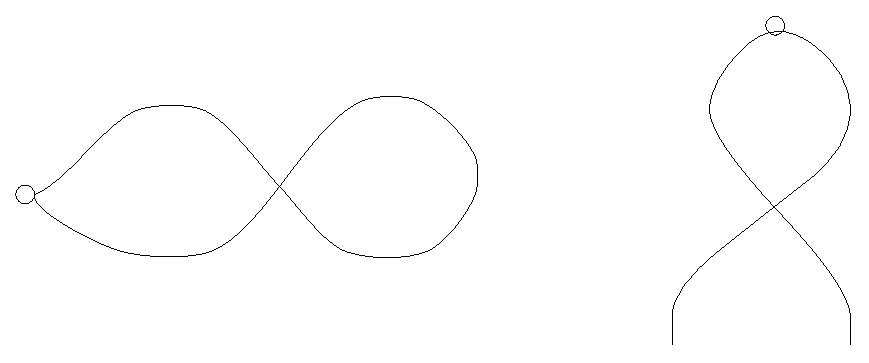
\epsfig{file=lec3-page7-1.eps,width=.4\linewidth} 
 
\end{center}


Let us call the first graph by $\Gamma_0$ and the second by $\Gamma_2$. 
The graph $\Gamma_0$ is quadratically divergent.
If we replace 
the usual propagator with the cutoff propagator, the integral will converge
to a $\L$-dependent constant of the form $gC_\L$,
where $C_\L$, which grows quadratically in $\L$. 

Now consider the graph $\Gamma_2$. 
 As usual, it is more
convenient to work in the momentum space, i.e. consider the Fourier 
transform of the term corresponding to this graph.
 Let $k_1,k_2,k$ be the corresponding momentum variables.
Then the Fourier transform of the  term corresponding to
$\Gamma_2$ is of the form $F_2\delta(k_1+k_2+k)$, where $F_2$ is a function
on the plane $k_1+k_2+k=0$. Set $k_1=r$, then $k_2=-r-k$ (on this plane).
Thus, $F_2=F_2(r,k)$, and its order $g$ correction is the amplitude 
of the Feynman diagram


\begin{center} 
 
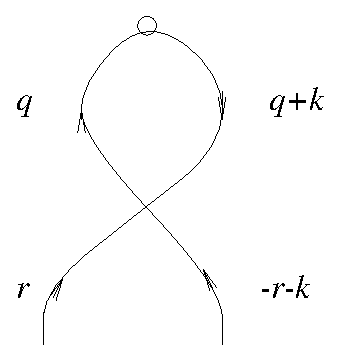
\epsfig{file=lec3-page7-2.eps,width=.25\linewidth} 
 
\end{center}


This amplitude is given by the integral
$$
I(k)=-\frac{g}{2}\int\frac{d^4q}{(2\pi)^4}\frac{1}{(q^2+m^2)((q+k)^2+m^2)}.
\leqno{(3.13)}
$$
This integral is logarithmically divergent. If we replace 
the usual propagator with the cutoff propagator, the integral will converge
to a function $I_\L(k)$, which has the asymptotic behavior
$$
I_\L(k)=-\frac{gA}{2}\ln(\L/\mu)+O(1), \L\to\infty
$$
where $A$ is a constant. 

This shows that if instead of $\phi^2/2$ we use the renormalized 
functional 
$$
\left(\frac{\phi^2}{2}\right)_\L:=\frac{\phi^2}{2}
(1+\frac{gA}{2}\ln(\L/\mu))-gC_\L,\leqno{(3.14)}
$$
the matrix elements will have a finite limit modulo $g^2$. 
Observe that the constant $\mu$ can be chosen arbitrarily, so the
renormalization is not canonical already in this case. 

{\bf 3.7. Stability of the classical field equations under quantization}

In a free theory, we know that the classical field equations are also 
satisfied quantum-mechanically. This means, if the classical equations
are $P\phi=0$, where $P$ is a linear differential operator, then 
the correlation functions in the quantum theory satisfy the equation
$P_x\<\phi(y_1)...\phi(y_r)\phi(x)\>=0$ outside of the diagonals 
$x=y_i$. For example, the Green's function $D(x-y)=\<\phi(x)\phi(y)\>$ 
is the fundamental solution of the equation $Pf=0$. 

 In an interacting theory, there are some problems.
Namely, since the classical field equations for an interacting theory are nonlinear
(e.g. (3.1)), they do not make sense quantum-mechanically in
the setting of Wightman axioms. However, in the OPE setting they
make sense in a suitable interpretation, 
and one can show that they are satisfied.

{\bf Remark.} We will say that the equation $F(\phi)=0$ is satisfied 
in quantum theory (where $F$ is a renormalized local functional) 
if the function $\<\phi(y_1)...\phi(y_r)F(\phi(x))\>$ vanishes
outside of the diagonals $x=y_i$.
 
We will show that the classical field equations are satisfied
in $\phi^4$ theory. 
Consider the space of classical local functionals of dimension 
$\le 3$, which are Poincare-invariant and odd under the symmetry
$\phi\to -\phi$. This space is 2-dimensional: it has 3 generators
$\phi^3$, $\Delta\phi$, and $\phi$, but they are linearly dependent,
since they satisfy relation (3.1). 

Now consider the quantum theory. Consider composite operators of
dimension $\le 3$, with the same invariance properties as above. 
In this space we have
renormalized operators $\Delta\phi$, $\phi$, $\phi^3$.
Our goal is to show that, like in the classical theory, they are linearly  
dependent. This is equivalent to the statement that $\phi$ satisfies
the field equation $C\phi^3=A\Delta\phi+B\phi$.

We will first prove the validity of the field equation for the theory
with the cutoff propagator, since in this theory we do not have 
divergence problems. In the cutoff theory, the classical field 
equation is 
$$
P_\L\phi=\frac{g}{3!}\phi^3,P_\L=(\Delta-m^2)(1-\frac{\Delta}{\L^2})^l.
\leqno{(3.15)}
$$

\vskip .02in

{\bf Proposition 3.3} Equation (3.15) holds in the quantum theory
with the cutoff propagator,
where $\phi$ and $\phi^3$ are regarded as composite operators. 

\vskip .02in

{\bf Proof.} Consider the correlation function $\<\phi(y_1)...\phi(y_r)
P_\L\phi(x)\>$. Consider the graph decomposition of 
this function. We should consider all possible graphs with 
$r$ external edges, any number of 4-valent internal vertices,
and a special vertex $v$ with 1 outgoing edge. These graphs 
can be of two kinds: 1) graphs in which $v$ connects to an external vertex;
2) graphs in which $v$ connects to an internal vertex. The sum over 
graphs of the first type is the corresponding correlation
function for the free theory, so it is supported on the 
union of diagonals $x=y_i$. Thus, outside of the diagonals 
we have to sum only over graphs of the second kind. 
But graphs of the second kind with $N$ external edges are in 1-1 
correspondence with usual Feynman graphs (without $v$) with 
$N+3$ external edges (this correspondence is obtained by biting off 
the vertex $v$ and the vertex it connects to). This shows that the sum
over graphs of the second kind is just
$\frac{g}{3!}\<\phi(y_1)...\phi(y_r)\phi^3(x)\>$. Thus, the field 
equation is satisfied, Q.E.D.

Proposition 3.3 shows that for any $\L$, the composite operator
$\frac{g}{3!}\phi^3$ is linearly dependent of composite operators
which are linear in $\phi$. This property has to be preserved
in the limit $\L\to\infty$. This shows that in the renormalized $\phi^4$ 
theory we have an equation $C\phi^3=P\phi$, where $P$ 
is a linear differential operator with constant coefficients, 
and $C$ is a constant.
Since the r.h.s. of this equation can only have terms of dimension $\le 3$,
the operator $P$ has to be of the form $A\Delta+B$. Thus 
in the quantum theory we have
the equation 
$$
C\phi^3=A\Delta\phi+B\phi\leqno{(3.16)}
$$

{\bf Remark.}
Of course, the constants $A,B,C$ are not uniquely defined, as they 
depend on the choice of the renormalization. The statement is only that
for any choice of renormalization, some nontrivial equation of the form 
(3.16) holds. In other words, the statement is that the space 
of Poincare invariant, 
odd composite operators of dimension $\le 3$ is 2-dimensional, 
i.e. has the same dimension as the corresponding space of classical 
local functionals. 

In general, one can consider the space of local functionals of
dimension $\le N$. Denote its dimension by $d(N)$. 
One can prove the following proposition.

\vskip .02in

{\bf Proposition 3.4} The space of composite operators 
of dimension $\le N$ is also equal to $d(N)$. 

\vskip .02in

Thus, all differential equations which are satisfied classically, have 
quantum analogues. 

{\bf 3.8. Operator product expansion in an interacting theory.}

In a free theory, once we defined composite operators, it was no problem 
to define the product of several of them supported at different points.  
The same is true in the interacting theory. Namely, if 
$\O_1,...,\O_N$ are renormalized composite operators, and $x_1,...,x_N\in V$ 
distinct points, then the correlation function 
$\<\phi(y_1)...\phi(y_r)\Theta(x_1)...\Theta(x_N)\>$ is just the 
coefficient of $\e_1...\e_N$ in the usual 
Schwinger function $\<\phi(y_1)...\phi(y_r)\>$ for the Lagrangian
$$
{\cal L}_{\e_1,...,\e_N}(\phi)={\cal L}(\phi)+\sum_{i=1}^N\e_i\O_i(\phi,x_i),\leqno{(3.17)}
$$
where $\e_i^2=0$. This Schwinger function is, by definition, the limit of
the corresponding function computed with the cutoff propagator. 
It is easy to see, by looking at Feynman diagrams,
 that this limit is always finite.

{\bf Remark.} Roughly speaking, this means that once we renormalized
each of the operators $\O_i$, we automatically renormalized
the product \[ \O_1(x_1)...\O_N(x_N), \ \ x_i\ne x_j.\]

Thus, now we are in as good shape as we were in the free
theory before we defined OPE. It turns out, we can define OPE in the
interacting theory as well. Namely, for any two composite operators 
$\O,\O'$ and for any $r\in \R$ 
there exists a finite collection of composite
operators $\O_1,...,\O_l$ such that 
$$
\O(x)\O(x')=\sum_{s=1}^l \O_s(x')D_s(x-x')+O(|x-x'|^r).
$$

We will show how to partially compute 
the OPE on examples. 

First we consider the product $\phi(x)\phi(x')$, and compute its 
asymptotics as $x\to x'$. 
In this case the expansion
is of the form: 
$$
\phi(x)\phi(x')=\phi^2_R(x')f(x-x')+h(x-x')+\text{ regular part },\leqno{(3.18)}
$$
where $\phi^2_R$ is the renormalized operator $\phi^2$
defined by (3.17).
(recall that $\phi^2_R$ is defined non-uniquely).
Let us find functions $f,h$.

The function $h(z)$ can be found by looking at the 
0-point function for the operator $\phi(x)\phi(x')$. 
Indeed, since $\<\phi^2_R(x)\>=0$ by the definition, 
we get $h(x-x')=\<\phi(x)\phi(x')\>$. 
If we compute the answer modulo $g^2$, we get 
no corrections to the free theory answer, so $h(z)=D(z)$
(see lecture 2).

Now let us find $f(z)$ (we remember that it is defined up to scaling
$f\to a(g)f$, where $a=1\text{ mod }g$). This 
function is found from the 2-point function of $\phi(x)\phi(x')$.
We have $f(z)=1+gf_1(z)+O(g^2)$. 
The only graph that contributes to $f_1(z)$ is 

\begin{center} 
 
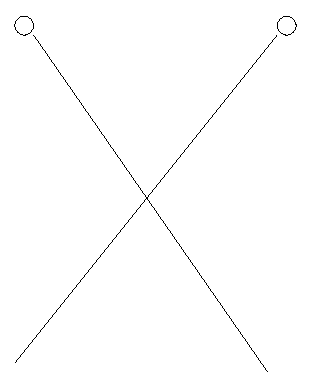
\epsfig{file=lec3-page10-1.eps,width=.2\linewidth} 
 
\end{center}

The amplitude of this graph (in the position space) is 
$$\begin{aligned}
g\int D(x-z)&D(x'-z)D(y_1-z)D(y_2-z)dz\\=&-\frac{gA}{2}\ln|\frac{x-x'}{\mu}|
D(y_1-x')D(y_2-x')\\&+\text{ regular part }\end{aligned}\leqno{(3.19)}
$$
($A$ is the same constant as in (3.17)). This shows that
$f_1(z)= -\frac{gA}{2}\ln|\frac{x-x'}{\mu}|$, and thus
$$\begin{aligned}
\phi(x)\phi(x')&=\phi^2_R(x')(1-\frac{gA}{2}\ln|\frac{x-x'}{\mu}|)
+D(x-x')\\&+\text{ regular part }+O(g^2).\end{aligned}\leqno{(3.20)}
$$

Now consider a more complicated operator product, for example 
\[ \phi_R^2(x)\phi_R^2(x').\] In this case the expansion is of the form
$$
\begin{aligned}
\phi_R^2(x)\phi_R^2(x')&
=\phi_R^4(x')f_1(x-x')+(\nabla\phi_R^2)(x')f_2(x-x')\\&
+\phi_R^2(x')f_3(x-x')+f_4(x-x')\\&+\text{ regular part },
\end{aligned}\leqno{(3.21)}
$$ 
where the subscript $R$ means ``renormalized composite operator''.
Of course the functions $f_1,...,f_4$ will depend on the choice 
of the renormalization, but they are well defined up to an upper
triangular linear transformation. 

For the sake of brevity we will only compute the expansion
modulo $O(|x-x'|^{-1})$. Thus, the functions $f_1,f_2$ can be ignored, 
and we only have to compute $f_3,f_4$ modulo $O(|x-x'|^{-1})$.

The function $f_4$ is defined canonically
up to multiplication by a scalar. 
As before, this function is computed using the 0-point function:
$f_4(x-x')=\<\phi^2_R(x)\phi^2_R(x')\>$. The only graph 
that contributes to the 1-st order in $g$ of $f_4$ is


\begin{center} 
 
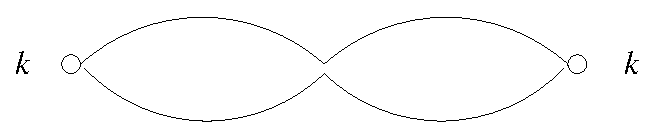
\epsfig{file=lec3-page11-1.eps,width=.4\linewidth} 
 
\end{center}

This shows that 
$$
f_4(z)=2D(z)^2+g\widehat{S(k)}+\text{ regular part }+O(g^2),
$$
where $S(k)$ is the amplitude (in the momentum space) of the above graph,
and hat denotes the Fourier transform. The function $S(k)$
equals $T(k)^2$, where $T(k)$ is the renormalized integral 
$$
T(k)=C\int_R \frac{dq}{(q^2+m^2)((k-q)^2+m^2)},
$$

{\bf Remark.} Since $T(k)$ is defined up to adding a constant, 
$f_4(z)$ is defined up to adding a multiple of 
$g\widehat{T(k)}$. Since $\widehat{T(k)}$ is proportional to $D^2(z)$
when $z\ne 0$, adding such multiple is equivalent to multiplying 
$f_4$ by $1+cg$. This freedom is natural, as $f_4$ is defined 
up to multiplying by $1+cg$. 

Now let us try to compute $f_3(z)$, which is also defined canonically 
up to a scalar. 
 For this purpose we should consider the 2-point function of
\[ \phi^2_R(x)\phi^2_R(x'),\] i.e.
\[ \<\phi(y_1)\phi(y_2)\phi^2_R(x)\phi^2_R(x')\>.\] 
We will work with the Fourier transform of this function,
which we denote by $F_2(p_1,p_2,q,q')$ (here $p_1,p_2,q,q'$
are the dual variables to $y_1,y_2,x,x'$).

We will try to compute the function $f_3(z)$
by looking at the asymptotic expansion of $F_2(p_1,p_2,q,r-q)$ 
as $|q|\to \infty$, and using the 
following fact from calculus:

\vskip 0.05in

{\bf Claim} 
Let $f$ be an $L^1$-function on an n-dimensional Euclidean space
$V$ whose Fourier transform $\hat f$ satisfies the inequality 
$|\hat f(q)|\le C|q|^{-n-N-\e}$, $\e>0$. Then $f\in C^n(V)$. 
 
\vskip 0.05in

By doing so we will be able 
to find $f_3(z)$ modulo $C^{\infty}$-functions,
which is all we want at this point. 

We have $f_3(z)=4D(z)+gf_3^1(z)$.
Looking at the Feynman diagram expansion of the 2-point 
function in the first order of $g$, we see terms of two kinds:
1) terms where the special vertices $v,v'$ are directly connected
with an edge; 2) terms where $v,v'$ are not connected. 

The only graph of the first kind that contributes to $f_3^1$ is

\begin{center} 
 
\epsfig{file=lec3-page11-2.eps,width=.2\linewidth} 
 
\end{center}


and the only graph of the second kind contributing to $f_3^1$ is


\begin{center} 
 
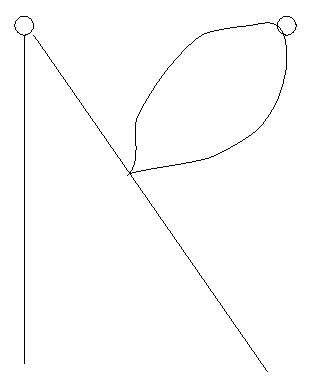
\epsfig{file=lec3-page11-3.eps,width=.2\linewidth} 
 
\end{center}


(this graph occurs 4 times, with 4 different labelings of vertices).
It is easy to check directly that both graphs contribute 
to $\hat f_3(q)$ a term of the form $Cq^{-2}\ln|q/\mu|+O(q^{-4+\e})$,
where $C$ is a constant. 
Thus, $f_3^1(z)$ is the Fourier transform of the function
$C\ln|q/\mu|/q^2$ modulo $O(|x-x'|)^{-1}$ and $O(g^2)$.    
As before, the constant $\mu$ depends on the choice of renormalization;
changing of this constant is equivalent to adding a multilple
of $D(z)$ to $f_3^1(z)$, which is the same as multiplying 
$f_3(z)$ by a scalar of the form $1+cg$.  

{\bf Remark:} Operator product expansion in conformal field theory.

In a 2-dimensional conformal field theory, the OPE of composite operators 
has especially simple form. In this case, $V=\C$, and the space of
functions on $V\setminus 0$ has a ``bigrading'': the function
$z^a\bar z^b$ has bidegree $(a,b)$ ($a-b\in\Z$).  
The space of composite operators also has a bigrading: to any
homogeneous operator $\O$ one assigns two numbers -- the holomorphic
dimension $d(\O)$ and antiholomorphic dimension $\bar d(\O')$
($d-\bar d\in \Z$). 
Therefore, if 
$\O(z)\O'(z')=\sum_k D_k(z-z')\O_k(z')$, then 
$D_k(z-z')$ has degree $(d_k,\bar d_k)$, where $d_k=d(\O)+d(\O')-
d(\O_k)$, $\bar d_k=\bar d(\O)+\bar d(\O')-
\bar d(\O_k)$. This implies that $D_k(z)=C_kz^{d_k}\bar z^{\bar d_k}$. 
Also, the action of the Virasoro algebra allows to reduce 
the problem of computing OPE of arbitrary operators to 
the problem of computing OPE for primary fields only, i.e. 
for fields which are highest weight vectors for the Virasoro algebra. 
In a rational conformal field theory, one has a chiral algebra
of symmetries (for example, an affine Lie algebra)
which is so big that there are only finitely many 
fields which are primary with respect to this algebra.     
This fact allows to treat a rational 2-dimensional conformal field theory 
in a purely algebraic setting, and reduce many of its problems to
problems in algebraic geometry. 

\end{document}


